%LV begin move all content to N9
%LV end move all content to N9
%LV begin insert content from N7
\chapter{Night 6: Eigenvalues and Eigenvectors}

%LV begin learning object insert
\begin{learningobjectives}
\emph{Concepts}
\bi
\item Compute the eigenvalues and eigenvectors of a $2\times 2$ matrix by hand
\item Compute the eigenvalues and eigenvectors of an $n \times n$ matrix using MATLAB
\item Describe the geometric meaning of eigenvalues and eigenvectors
\item Use eigenvectors to compute and interpret directions of variation in data
\ei
\emph{MATLAB skills}
\bi
\item Compute the eigenvectors and eigenvalues of a given matrix
\item From a given dataset, set up the relevant matrices and compute the covariance matrix of the dataset.
\ei
\end{learningobjectives}
%LV end learning objectives insert


\subsection{What is this about?}

The big ideas of this assignment are eigenvectors and eigenvalues. Recall that when you multiply a vector by a matrix, the resulting vector usually points in a different direction. An eigenvector of a square matrix is a vector which does not change direction when multiplied by that matrix. It can only change in length. The eigenvalue corresponding to this eigenvector is the scale factor that is applied to that eigenvector as a result of the matrix multiplication.  Therefore, the eigenvector of a matrix points in a special direction -- its a direction that is not modified by the linear transformation associated with that matrix. This is an idea that we will keep coming back to in a number of different ways throughout QEA (including next semester). The ideas contained here can be applied in many ways (many of which we won't get to until next semester) such as
\begin{itemize}
\item Directions of greatest variation in data.
\item Natural co-ordinates of systems.
\item Frequency response of filters.
\item Analysis of dynamical systems.
\end{itemize}


\subsection{Reference Material}

\begin{itemize}
\item \href{https://www.youtube.com/watch?v=PFDu9oVAE-g}{Eigenvalues and Eigenvectors by 3Blue1Brown} (watch first 14 mins)
\item \href{http://tutorial.math.lamar.edu/Classes/DE/LA_Eigen.aspx}{Paul's Online Notes. Review : Eigenvalues and Eigenvectors}
\item \href{https://www.youtube.com/watch?v=G4N8vJpf7hM}{Intro to eigenvectors by PatrickJMT}
\item \href{https://www.youtube.com/watch?v=IdsV0RaC9jM}{Calculating eigenvalues and eigenvectors of a $2\times 2$ matrix by PatrickJMT.}
\end{itemize}

\section{Calculating Eigenvalues and Eigenvectors of Matrices }

Recall from class that $\lambda$ is an eigenvalue of a matrix $\A$ with corresponding eigenvector $\v$ if $\A\v=\lambda\v$. Geometrically, this means that the matrix $\A$ doesn't change the direction of $\v$, it simply scales it by a factor of $\lambda$.

Given a square matrix, how can we find its eigenvalues and eigenvectors? In class, we calculated these by hand for the special case of diagonal matrices, and now we will move to generic $2\times 2$ matrices. For general square matrices which are larger than $2\times 2$, we will use MATLAB's $\texttt{eig}$  to compute the eigenvalues and eigenvectors.

\subsection{Finding eigenvalues}

So far we've dealt with matrices for which it is possible to think your way to the eigenvalues. For general matrices, this is rarely the case, and we need a method that is foolproof. The method most widely adopted involves the determination of an algebraic equation for the eigenvalues, usually known as the \textit{characteristic} equation. For this reason, eigenvalues are often known as characteristic values. 

Let's start with an example. Consider the matrix
\[ \A = \twobytwo{18}{-2}{12}{7} \]
The definition of an eigenvalue and eigenvector imply that we are seeking $\lambda$ and $\v$ which satisfy
\[ \A \v = \lambda \v. \]
We subtract $\lambda \v$ from both sides
\[ \A \v - \lambda \v = \mathbf{0} \]
and then factor the left hand side to give
\[ (\A - \lambda \mathbf{I}) \v = \mathbf{0} \]
For this example we have
\[ \A - \lambda \mathbf{I} = \twobytwo{18-\lambda}{-2}{12}{7-\lambda}. \]

We are only interested in $\mathbf{v}$ that are nonzero, i.e., $\v$ is not the vector of all zeroes. (This is because $\v=\mathbf{0}$ is always a solution to $\A\v=\lambda\v$ for any $\A$ and any $\lambda$, so it's not very interesting or informative.) Assuming $\v$ is nonzero implies that the matrix $(\A - \lambda\mathbf{I})$ is not invertible. Why? If $(A-\lambda\mathbf{I})$ were invertible, then we could rearrange the equation to get
$$\v = (\A - \lambda\mathbf{I})^{-1}\mathbf{0} = \mathbf{0}$$
which contradicts our assumption that $\v\neq\mathbf{0}$. THerefore, $(\A - \lambda \mathbf{I})$ is not invertible.

Since $(\A - \lambda \mathbf{I})$ is not invertible, it must have determinant zero. In other words,
\[\det(\A - \lambda \mathbf{I}) = 0. \]

In our example, this implies that
\[ \det(\A - \lambda \mathbf{I}) = (18-\lambda)(7 - \lambda) + 24 =0.\]

This is called the characteristic equation:
\[ (18-\lambda)(7 - \lambda) + 24 = 0 \]
or, rearranged,
\[\lambda^2 - 25 \lambda + 150 = 0.\]
The characteristic equation is a polynomial with the variable $\lambda$ that arises by setting the determinant of $(\A-\lambda\mathbf{I})$ equal to zero. The solutions to this polynomial give the eigenvalues $\lambda$. In our example, the polynomial can be factored
\[(\lambda - 15)(\lambda - 10) = 0 \]
so that gives eigenvalues $\lambda_1 = 10$ and $\lambda_2 = 15$. (We could use the quadratic formula if necessary.)

Let's retrace our steps: If $\lambda$ is either 10 or 15, then the determinant of $(\A - \lambda\mathbf{I})$ is zero. This implies that $(\A - \lambda\mathbf{I})$ is not invertible, so we can look for nonzero solutions $\v$ to $(\A - \lambda\mathbf{I})\v = \mathbf{0}$ and those $\v$ are eigenvectors associated to the eigenvalue $\lambda$.

In summary, here's the general procedure for finding the eigenvalues of a matrix:
\begin{enumerate}
    \item Rearrange $\A\v=\lambda\v$ to get $(\A-\lambda\mathbf{I})=\mathbf{0}$.
    \item Compute the determinant of $(\A-\lambda\mathbf{I})$. 
    \item Since the matrix is not invertible, we set that determinant equal to zero: $\det(\A-\lambda\mathbf{I})=0$. This gives a polynomial in $\lambda$, known as the characteristic equation.
    \item Solve the polynomial for the roots $\lambda$. Those are the eigenvalues.
    
\end{enumerate}

\begin{prob}
\begin{enumerate}
    \item You already know that the eigenvalues of a diagonal matrix are just the entries on the diagonal. Using the above procedure, confirm that
\[ \A = \twobytwo{2}{0}{0}{-3} \]
has eigenvalues $\lambda_1=2$ and $\lambda_2=-3$.
\item Notice that one of the eigenvalues is positive and one is negative. The eigenvector associated with $\lambda_1=2$ is $\v_1=\twobyone{1}{0}$ and the eigenvector associated with $\lambda_2=-3$ is $\v_2=\twobyone{0}{1}$. Plot $\v_1,\v_2,\A\v_1$ and $\A\v_2$. What affect does the negative sign in the eigenvalue have? In other words, what is the difference between a negative and positive eigenvalue?
\end{enumerate}
\end{prob}
\begin{sol}
\begin{enumerate}
\item First we find
$$\A - \lambda\mathbf{I} = \twobytwo{2-\lambda}{0}{0}{-3-\lambda}.$$
And then we compute the determinant
$$\det(\A-\lambda\mathbf{I})=(2-\lambda)(-3-\lambda).$$
Setting this equal to zero produces the characteristic equation,
$$(2-\lambda)(-3-\lambda)=0$$
whose roots are, in fact, $\lambda_1=2$ and $\lambda_2=-3$.
\item Here's a plot of $\v_1,\v_2,\A\v_1$ and $\A\v_2$:
    \begin{center}
    \begin{tikzpicture}[scale=0.6]
    \draw [->,gray!50!black] (0,0)--(0,3) node[above]{$y$};
    \draw [->,gray!50!black] (0,0)--(3,0) node[right]{$x$};

    \draw [->,red,thick] (0,0)--(0,1) node[midway,left] {$\mathbf{v_2}$};
    \draw [->,blue] (0,0)--(0,-3) node[midway,left] {$\mathbf{\A\v_2}$};
    \draw [->,red,thick] (0,0)--(1,0) node[midway,below] {$\mathbf{\v_1}$};
    \draw [->,blue] (0,0)--(2,0) node[midway,above] {$\mathbf{\A\v_1}$};
    \end{tikzpicture}
    \end{center}
    When the eigenvalue is negative, the eigenvector is reversed in direction and then scaled.
\end{enumerate}
\end{sol}

It's worth noting that eigenvalues come in more flavors than positive or negative. They can also be complex numbers. For now, will focus on matrices with real eigenvalues, but if you're curious about the complex case, you can learn about it~\href{https://www.google.com/url?sa=t&rct=j&q=&esrc=s&source=web&cd=17&cad=rja&uact=8&ved=2ahUKEwiX1J_x8cTnAhULxVkKHd2GBAQ4ChAWMAZ6BAgEEAE&url=https%3A%2F%2Fcanvas.harvard.edu%2Ffiles%2F5645480%2Fdownload%3Fdownload_frd%3D1&usg=AOvVaw3YkWN7j8kjPcIgHW4GaRH3}{in this worksheet} (ignore the first page).

\subsection{Eigenvalues in terms of the trace and determinant}

The steps we took just in the previous sections will work for any matrix, so let's apply it to the most general $2\times2$ matrix
\[ \A = \twobytwo{a}{b}{c}{d} \]
Again we seek $\lambda$ and $\v$ so that
\[ \A \v = \lambda \v \]
or equivalently
\[ (\A - \lambda \mathbf{I})\v = \mathbf{0} \]
Non-zero solutions for $\v$ exist when
\[ \det(\A - \lambda \mathbf{I}) = 0 \]
so in the general case the characteristic equation is
\[ (a-\lambda)(d-\lambda) - bc = 0 \]
Expanding and simplifying gives
\[\lambda^2 - (a+d) \lambda + (ad - bc) = 0 \]
which is a second-order polynomial in $\lambda$ with two coefficients. Notice that the last one is just $det(\A)$ and the middle one involves the sum of the diagonal entries of $\A$, which is known as the trace of $\A$ or $tr(\A)$ for short. The characteristic equation is therefore
\[ \lambda^2 - tr(\A) \lambda + det(\A) = 0 \]

Finally, let's consider the solutions of the characteristic equation for a 2x2 matrix. Using the quadratic formula we have
\[ \lambda = \frac{tr(\A) \pm \sqrt{tr(\A)^2 - 4 det(\A)}}{2} \]
If you recall all the work you did in school with the solutions to the quadratic, you will notice that there are two solutions as expected, one for each eigenvalue. Furthermore, the solutions may be \textit{complex} if
\[ tr(\A)^2 - 4 det(\A) < 0. \]

\begin{prob}
Determine the trace and determinant of the following 2x2 matrices and then write down the corresponding characteristic equation. Solve the characteristic equation to find the eigenvalues.
\begin{enumerate}
\item \[ \A = \twobytwo{1}{2}{2}{1} \]
\item \[ \A = \twobytwo{1}{2}{3}{2} \]
\end{enumerate}
\end{prob}
\begin{sol}
\begin{enumerate}
    \item Since $\text{tr}(\A)=2$ and $\det(\A)=-3$, we have
    \[\lambda^2 - 2 \lambda - 3 = 0 \]
    so $\lambda_1=-1$ and $\lambda_2=3$.
    \item Since $\text{tr}(\A)=3$ and $\det(\A)=-4$, we have
    \[\lambda^2 - 3 \lambda - 4 = 0 \]
    so $\lambda_1=-1$ and $\lambda_2=4$.
\end{enumerate}
\end{sol}

\begin{prob}
\textbf{Optional problem} if you're interested in further exploring the relationship between the trace, determinant, and eigenvalues.
\begin{enumerate}
\item Use the solutions of the characteristic equation to prove that $\lambda_1 + \lambda_2 = tr(\A)$.
\item Use the solutions of the characteristic equation to prove that $\lambda_1 \lambda_2 = det(\A)$.
\item Use the solutions of the characteristic equation to prove that the eigenvalues of a symmetric $2\times 2$ matrix are real.
\end{enumerate}
\end{prob}
\begin{sol}
\begin{enumerate}
    \item 
    \begin{align*}
    \lambda_1+\lambda_2 &= \frac{tr(\A) + \sqrt{tr(\A)^2 - 4 det(\A)}}{2}+\frac{tr(\A) - \sqrt{tr(\A)^2 - 4 det(\A)}}{2}\\
    &=\frac{tr(\A)}{2}+\frac{tr(\A)}{2}=tr(\A)
    \end{align*}
    \item
    \begin{align*}
    \lambda_1 \lambda_2 &= \Big(\frac{tr(\A)}{2}\Big)^2+\Big(\frac{tr(\A)}{2}\Big)\Big( \sqrt{tr(\A)^2 -4 det(\A)}\Big)\\
    &-\Big(\frac{tr(\A)}{2}\Big)\Big( \sqrt{tr(\A)^2 - 4 det(\A)}\Big)-\Big(\frac{\sqrt{tr(\A)^2 - 4 det(\A)}}{2}\Big)^2\\
    &=\frac{tr(\A)^2}{4}-\frac{tr(\A)^2 - 4 det(\A)}{4}\\
    &=det(\A)
    \end{align*}
\item Symmetric means $b=c$ and real $\lambda$ means:
\[tr(\A)^2 - 4 det(\A)\ge 0\]
\[(a+d)^2-4(ad-bc)\ge 0 \]
\[(a+d)^2-4(ad-bc)=a^2+d^2+2ad-4ad+4bc=a^2+d^2-2ad+4b^2=(a-d)^2+4b^2\]
Squares of real numbers are positive, so $tr(\A)^2 - 4 det(\A) \ge 0$ and the eigenvalues $\lambda$ are real.
\end{enumerate}
\end{sol}

\subsection{Finding Eigenvectors}

In the example in the previous section, we discovered that the eigenvalues of 
\[ \A = \twobytwo{18}{-2}{12}{7} \]
are $\lambda_1 = 10$ and $\lambda_2=15$. How do we find the corresponding eigenvectors $\v_1$ and $\v_2$?

First, let's find the eigenvector corresponding to $\lambda_1=10$. Remember that we knew $\lambda_1$ was an eigenvalue because it solved the characteristic equation, i.e., $\det(\A-\lambda_1\mathbf{I})=\mathbf{0}$.
This is important because it implies $(\A-\lambda_1\mathbf{I})$ is non-invertible, and therefore, there exists a nonzero vector $\v_1$ such that $(\A-\lambda_1\mathbf{I})\v_1=\mathbf{0}$. But it's not enough just to know that such a vector exists, we want to know exactly what it is.

In our running example, this means we are looking for $\v_1$ such that
$$(\A-\lambda_1\mathbf{I})\v_1 = \twobytwo{18-10}{-2}{12}{7-10}\v_1 = \twobytwo{8}{-2}{12}{-3}\v_1 = \mathbf{0}.$$
Let's write $\v_1$ in terms of its components
$$\v_1 = \twobyone{a}{b},$$
to get the equation
$$\twobytwo{8}{-2}{12}{-3}\twobyone{a}{b} = \twobyone{0}{0}.$$
This gives us two equations
$$8a-2b=0 \ \text{ and } 12a-3b=0.$$
But these equations provide the same information: they both imply that $b = 4a$. This is because $(\A-\lambda_1\mathbf{I})$ is not invertible, so the rows are linear dependent. The system of linear equations implied by $(\A-\lambda_1\mathbf{I})\v_1=\mathbf{0}$ has infinitely many solutions of the form $\twobyone{a}{4a}$ for any $a$. Letting $a=1$, we get $\v_1=\twobyone{1}{4}$.

If we let $a=5$, we would have the eigenvector $\twobyone{5}{20}$. This hints at an important fact about eigenvectors: \textit{we only care about an eigenvector's direction, not its length}. So we could have chosen $\v_1$ to be any vector pointing the same direction as $\twobyone{1}{4}$ (such as $\twobyone{5}{20}$ or $\twobyone{-2}{-8}$). We often speak about ``the'' eigenvector corresponding to an eigenvalue, but only the direction of the eigenvector is unique, not the length.

\begin{prob}
Using the basic eigenvalue/eigenvector equation
$$\A\v = \lambda\v$$
show that if $\v$ is an eigenvector for $\lambda$, then $c\v$ is also an eigenvector for $\lambda$, where $c$ is any constant.
\end{prob}
\begin{sol}
Using the fact that $\A\v=\lambda\v$, we see that
$$\A(c\v) = c\A\v = c\lambda\v = \lambda(c\v)$$
and therefore $c\v$ is also an eigenvector.
\end{sol}

\begin{prob}
We can always check that $\lambda_1$ and $\v_1$ are the corresponding eigenvalue and eigenvector for the matrix $\A$ by plugging them into the equation $\A\v_1 = \lambda_1\v_1$ and verifying that it holds.

Use this procedure to check that $\lambda_1=10$ and $\v_1=\twobyone{1}{4}$ are the corresponding eigenvalue and eigenvector for $\A = \twobytwo{18}{-2}{12}{7}$.
\end{prob}
\begin{sol}
First we compute the left-hand side
$$\A\v_1 = \twobytwo{18}{-2}{12}{7}\twobyone{1}{4} = \twobyone{10}{40}$$
and the right-hand side
$$\lambda_1\v_1 = 10\twobyone{1}{4} = \twobyone{10}{40}.$$
Fortunately, they are equal.
\end{sol}

\begin{prob}
Continuing the example above, with $$\A = \twobytwo{18}{-2}{12}{7}$$ find the eigenvector that corresponds to the eigenvalue $\lambda_2 = 15$.
\end{prob}
\begin{sol}
First we compute
$$\A - \lambda_2\mathbf{I} = \twobytwo{18-15}{-2}{12}{7-15} = \twobytwo{3}{-2}{12}{-8}.$$
Now, letting $\v_2=\twobyone{a}{b}$, we are trying to solve
$$\twobytwo{3}{-2}{12}{-8}\twobyone{a}{b} = \twobyone{0}{0},$$
which produces the equations
$$3a-2b = 0 \ \text{ and } \ 12a-8b = 0.$$
(These equations give the same information since the rows of $(\A-\lambda_2\mathbf{I})$ are linearly dependent.) This gives $b = \frac{3}{2}a$, so $\v_2=\twobyone{a}{\frac{3}{2}a}$ for any value of $a$. Picking $a=2$, we have $\v_2 = \twobyone{2}{3}$.
\end{sol}

\subsection{More Eigen-stuff}

\begin{prob}\label{EigenvectorQuestion} 
Determine the eigenvalues and eigenvectors of the following 2x2 matrices.
\begin{enumerate}
\item \[ \A = \twobytwo{4}{2}{1}{3} \]
\item \[ \A = \twobytwo{1}{2}{3}{2} \]
\end{enumerate}
\end{prob}
\begin{sol}
\begin{enumerate}
    \item \[ \lambda = 5,2\] and \[ \v = \twobyone{2}{1},\twobyone{-1}{1}\]
    \item \[ \lambda = -1,4\] and \[ \v = \twobyone{-1}{1},\twobyone{2}{3}\]
\end{enumerate}
\end{sol}

\begin{prob}\label{OneDirectionQuestion}  
We have two vectors,
    \begin{align}
        \mathbf{n} = \twobyone{-1}{1}
    \end{align}
    but
    \begin{align}
        \mathbf{z} = \twobyone{-1}{1.01}
    \end{align}
    In other words, the vectors  $\mathbf{n}$ and $\mathbf{z}$ point in a very similar direction, but are not perfectly aligned.
    Now consider a  matrix $\mathbf{S}$ given by

    \begin{align}
    \mathbf{S} = \twobytwo{2}{1}{1}{2}
    \end{align}

    \begin{enumerate}
    \item On the same axes, plot the vectors $\mathbf{n}$ and $\mathbf{z}$ using MATLAB.
    \item Suppose that $\mathbf{n}$ and $\mathbf{z}$ are transformed by $\mathbf{S}$. On the same axes as in the previous part, plot the vectors $\mathbf{S}\mathbf{n}$ and $\mathbf{S}\mathbf{z}$ using MATLAB.
    \item Now, we shall see what happens to these vectors under repeated transformations by $\mathbf{S}$. On the same axes as in the previous part, plot the vectors $\mathbf{SS}\mathbf{n}$ and $\mathbf{SS}\mathbf{z}$ using MATLAB.
    \item On the same axes as in the previous part, plot the vectors $\mathbf{SSS}\mathbf{n}$ and $\mathbf{SSS}\mathbf{z}$ using MATLAB.
    \item On the same axes as in the previous part, plot the vectors $\mathbf{SSSS}\mathbf{n}$ and $\mathbf{SSSS}\mathbf{z}$ using MATLAB.

    \item You should find that $\mathbf{n}$ is unaffected by the transformation by $\mathbf{S}$, but $\mathbf{z}$ on the other hand moves farther and farther away. In other words, under repeated transformations by $\mathbf{S}$, $\mathbf{z}$ grew further and further apart from his four friends.  Explain what you see in terms of eigenvalues and eigenvectors.
    \end{enumerate}
\end{prob}
\begin{sol}
See Figure \ref{Sblub}. $\mathbf{n}$ is an eigenvector of $\mathbf{S}$ with an eigenvalue of 1, so it is unchanged by the transformation $\mathbf{S}$. However, $\mathbf{z}$ is not an eigenvector of $\mathbf{S}$, so it changes each time the transformation $\mathbf{S}$ is applied, and the change accelerates as it diverges from the eigenvector $\mathbf{n}$.

\begin{center}
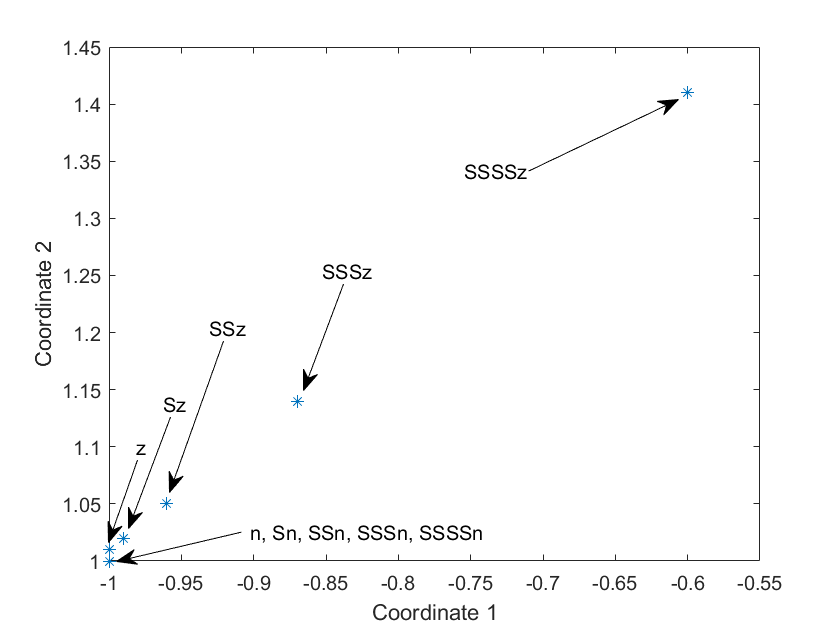
\includegraphics[width=11cm]{FacesNight5/figs/SSSSz.png}
\captionof{figure}{Plot for Exercise 9.}
\label{Sblub}
\end{center}
\end{sol}

\section{Properties and Applications of Eigenvalues and Eigenvectors}
While most of our work on eigenvalues and eigenvectors has focused on 2D vectors and $2\times 2$ matrices, these ideas extend to higher dimensions as well. The eigenvalues and eigenvectors can be found by solving the characteristic polynomial, or by using the MATLAB \texttt{eig} function.

A few words about \texttt{eig} are in order. The following command
\begin{verbatim}
>> [V,D] = eig(A)
\end{verbatim}
will return two matrices. The columns of the matrix $V$ are the eigenvectors. $D$ is a diagonal matrix, with the eigenvalues on the diagonal. The first eigenvector is in the first column of $V$ and has a corresponding eigenvalue in the first diagonal entry of $D$. Each eigenvector is normalized to have a magnitude of 1. The eigenvalues will often "appear" to be sorted according to their size, but this is not necessarily true, and is simply an artifact of the algorithm used to compute them. See the documentation in MATLAB for more details.

Consider an $n\times n$ matrix $\A$. The characteristic polynomial will be a polynomial of degree $n$ in $\lambda$, i.e., it will have the form
$$c_n\lambda^n + \cdots + c_1\lambda + c_0 = 0$$
where $c_i$ are constants. This polynomial will have $n$ roots, although some of those roots might be the same (e.g., both roots of the polynomial $\lambda^2 + 2\lambda + 1=0$ are $-1$, so we say $\lambda_1=-1$ and $\lambda_2=-1$.) This means that an $n\times n$ matrix has $n$ eigenvalues $\lambda_1, \lambda_2, \cdots, \lambda_n$, where its possible that some eigenvalues are equal.

The following are properties of the eigenvalues (some of these are $n$-dimensional extensions of what you already saw for 2 dimensions).
\begin{itemize}
\item $\mbox{Tr}(\A) = \lambda_1+\lambda_2 + \cdots +\lambda_n$\\\
\item $\mbox{det}(\A)= \lambda_1\lambda_2  \cdots  \lambda_n$\\\
\item $\A$  is invertible if and only if all eigenvalues are nonzero.
\item If the eigenvalues are distinct (none are equal) then the corresponding eigenvectors are linearly independent.
\item If a matrix is symmetric, i.e., $\A = \A^T$, then its eigenvalues are real and its eigenvectors are orthogonal to each other.
\end{itemize}

\begin{prob}
In this problem, you will get some practice seeing some of the properties above in action. First, create a $3\times 3$ matrix in MATLAB, with any values you'd like and call it \texttt{A}. Alternatively, you can ask MATLAB to generate a $3\times 3$ matrix with random entries using \texttt{A = randn(3, 3);}.

    \begin{enumerate}
    \item Use MATLAB's \texttt{eig} function to get the eigenvalues and eigenvectors of the matrix.
    \item Using MATLAB's \texttt{trace} function, confirm that the trace equals the sum of the eigenvalues.
    \item Using MATLAB's \texttt{det} function, confirm that the determinant equals the product of the eigenvalues, and explain why a square matrix is invertible if and only if all its eigenvalues are nonzero.
    \item Generate a new matrix $\mathbf{B} = \mathbf{A}^T\mathbf{A}$ which must be symmetric. Find its eigenvalues and eigenvectors using \texttt{eig}, and verify that the eigenvectors are orthogonal.
    \end{enumerate}
\end{prob}
\begin{sol}
\begin{enumerate}
    \item \texttt{A=randn(3,3);[V,D]=eig(A)}
    \item \texttt{trace(A)-sum(diag(D))}
    \item \texttt{det(A)-prod(diag(D))} 

The product of all eigenvalues equals the determinant of the matrix. If any eigenvalue is zero, the determinant is zero and the matrix is non-invertible; if all eigenvalues are nonzero, the determinant is nonzero and the matrix is invertible.
\item  \texttt{B=A'*A;[V D]=eig(B);V'*V} gives the identity matrix, showing that the eigenvectors are orthogonal (and of unit length).
\end{enumerate}
\end{sol}


% \todo[inline]{more multivariable calculus! a lot of it!}
% The eigenvalues of the Hessian matrix of a function have useful properties as well. In almost all cases the Hessian will be symmetric (equality of mixed partial derivatives), and so its eigenvalues are real. If we evaluate the Hessian at a critical point, and then find the eigenvalues, the critical point has the following properties:
% \begin{itemize}
% \item If all eigenvalues are positive, the critical point is a minimum.
% \item If all eigenvalues are negative, the critical point is a maximum.
% \item If the eigenvalues are a mix of positive and negative values, the critical point is a saddle point.
% \end{itemize}
% In the case of a saddle, the eigenvectors of the Hessian tell about the directions in which the function is increasing most rapidly (positive eigenvalue) or decreasing most rapidly (negative eigenvalue). The proof of this is a little bit beyond the scope of this exercise, but we included it here as an example of the applications of eigenvalues in a context that you are already familiar with from the last assignment. You can solve this problem combining techniques for finding the Hessian from last week and on how to find eigenvalues from this exercise.

% Instead (and this is completely optional), if you would like to solve this problem using vector derivatives, you can watch the following videos, and convince yourself that the second derivative with respect to a vector is equivalent to a Hessian matrix.

% \begin{itemize}
% \item \href{https://www.youtube.com/watch?v=iWxY7VdcSH8}{How to differentiate with respect to a vector Part 1 by Ben Lambert}
% \item \href{https://www.youtube.com/watch?v=uoejt0FCWWA}{How to differentiate with respect to a vector Part 2 by Ben Lambert}
% \end{itemize}


% \begin{prob}
% \label{HessianQuestion}
% Consider the following  function of the vector $\x = \twobyone{x_1}{x_2}$.
% $$
% f(\mathbf{x}) = (\mathbf{x}-\mathbf{b})^T\mathbf{A}(\mathbf{x}-\mathbf{b})
% $$
% where
% $$\mathbf{A} = \twobytwo{1}{1}{3}{-1}$$
% $$
% \mathbf{b} = \twobyone{1}{2}
% $$

% \begin{center}
% \includegraphics[scale=0.6]{FacesNight5/figs/Saddle_point_surf.pdf}
% \captionof{figure}{Surface plot of $f(\x)$. }
% \label{figSaddlePointSurf}
% \end{center}

% \begin{center}
% \includegraphics[width=11cm]{FacesNight5/figs/Saddle_point_contour.pdf}
% \captionof{figure}{Contour plot of $f(\x)$. }
% \label{figSaddlePointContour}
% \end{center}

% Figure \ref{figSaddlePointSurf} is a surface plot of  $f(\x)$ plotted in the range $[-10,10]$ for both $x_1$ and $x_2$, with the red dot representing the only critical point of the function Figure \ref{figSaddlePointContour} is a contour plot of $f(\x)$. We've also provided a MATLAB figure file which you can open and use the "Rotate 3D" feature to view the surface plot from different angles.

% \begin{enumerate}
% \item Find the gradient of $f(\x)$.
% \item Find the critical point of this function, and confirm that it matches the figures.
% \item Find the Hessian of $f(\x)$ and evaluate it at the critical point.
% \item Compute the eigenvalues and eigenvectors of the Hessian at the critical point.
% \item Verify that the critical point is a saddle point, and that the eigenvectors match the orientation of the saddle. What do the eigenvalues tell you?
% \end{enumerate}
% \end{prob}
% \begin{sol}
% \begin{enumerate}
%     \item Use the product rule or whatever: \[ \nabla f = \twobyone{2x_1+4x_2-10}{4x_1+-2x_2}\]
%     \item Evaulate $\nabla f=0$: \[ \twobyone{1}{2} \]
%     \item \[Hf=\twobytwo{2}{4}{4}{-2}\] everywhere, including the critical point.
%     \item Use quadratic formula to find eigenvalues of $\sqrt{20}$ and $-\sqrt{20}$ with corresponding eigenvectors of:
% \[ \twobyone{\frac{1+\sqrt{5}}{2}}{1} \] and \[ \twobyone{\frac{1-\sqrt{5}}{2}}{1} \]
% \item The eigenvalues of the Hessian are a mix of positive and negative values, so the critical point is a saddle. The eigenvector corresponding to the positive eigenvalue points in the direction of fastest increase of the function, while the eigenvector corresponding to the negative eigenvalue points in the direction of fastest decrease.
% \end{enumerate}
% \end{sol}

% \newpage

\section{Eigenvalues and Eigenvectors in Data Analysis}

In the last class you worked on examples involving correlation matrices. Here we will look at covariance matrices, which are related to correlation matrices, except that the entries are not normalized by the standard deviations of the variables. You can think of covariance matrices as measuring the relationship between random quantities, but without normalization. Thus, information about how small or large these data values are will still be preserved in the covariance matrix.

Suppose that  we have two different data variables $x$ and $y$ (e.g. corresponding to temperatures in Boston and Sao Paolo), with $x_i$ and $y_i$ being different values in the data set we can define a a matrix $\mathbf{A}$ as follows:
\begin{align*}
\mathbf{A} = \frac{1}{\sqrt{N-1}} \begin{pmatrix}
    {x_1-\mu_x} & {y_1-\mu_y}\\
   {x_2-\mu_x} &  {y_2-\mu_y}\\
    {x_3-\mu_x} & {y_3-\mu_y}\\
    \vdots & \vdots \\
    x_N - \mu_x & y_N - \mu_y
  \end{pmatrix}
\end{align*}
where $\mu_x$ is the mean  of the first column, and $N$ is the number of samples (rows).  The covariance matrix of $x$ and $y$ is $\mathbf{R} = \mathbf{A}^T \mathbf{A}$. You can think of the entries of this matrix as storing the un-normalized correlations between the temperatures. Because $\mathbf{R}^T = \mathbf{R}$, this matrix is symmetric, and hence has orthogonal eigenvectors.

The eigenvectors and eigenvalues of $\mathbf{R}$ tell us something about how the data are distributed.  The eigenvector corresponding to the largest eigenvalue of $\mathbf{R}$, which is also called the \emph{principal eigenvector} of $\mathbf{R}$ points in the direction with the largest variation in the data. The eigenvector corresponding to the second largest eigenvalue points in the direction orthogonal to the principal eigenvector in which there is the second largest amount of variation in the data, and so on (if you have more than 2 dimensional data). The square-root of the eigenvalues tells you about the amount of variation there is in each of those directions. Of course when you only have two different variables in the data set, the matrix $\mathbf{R}$ has only 2 orthogonal eigenvectors.

To illustrate, consider Figure \ref{figBostonSaoPaolo} which shows the centered (mean subtracted) temperatures of Boston vs Sao Paolo. We have also plotted  the two eigenvectors, scaled by the square-root of their corresponding eigenvalues, to illustrate the relative variation of the data along the directions of the two eigenvectors. Notice that the principal eigenvector is in the direction of greatest variation in the data. Figure \ref{figBostonWashington} is a similar plot with the temperatures of Boston and Washington DC instead.

The proof of this is optional and will be introduced in the future.

\begin{center}
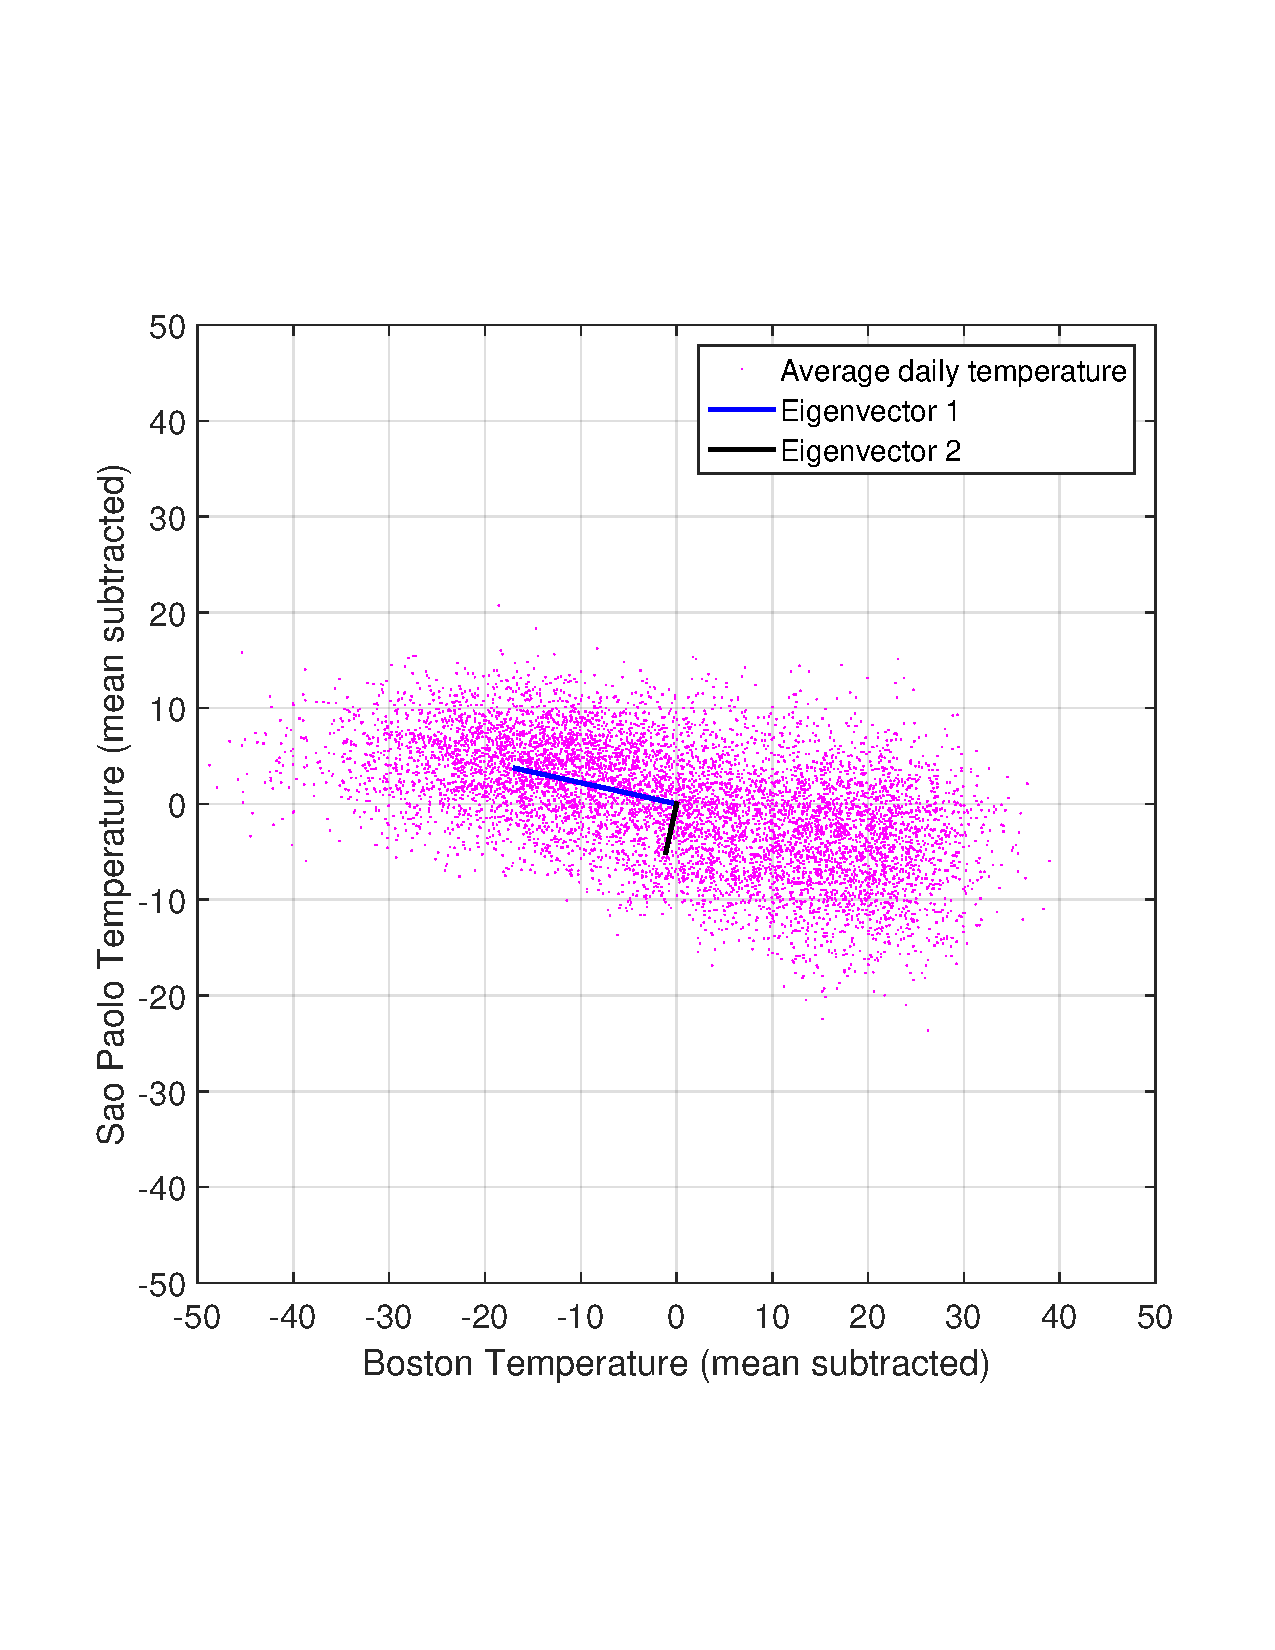
\includegraphics[width=0.75\textwidth]{FacesNight5/figs/BostonSaoPaoloCentered.pdf}
\captionof{figure}{Centered average daily temperatures of Boston vs Sao Paolo, with the eigenvectors of the covariance matrix.}
\label{figBostonSaoPaolo}
\end{center}

\begin{center}
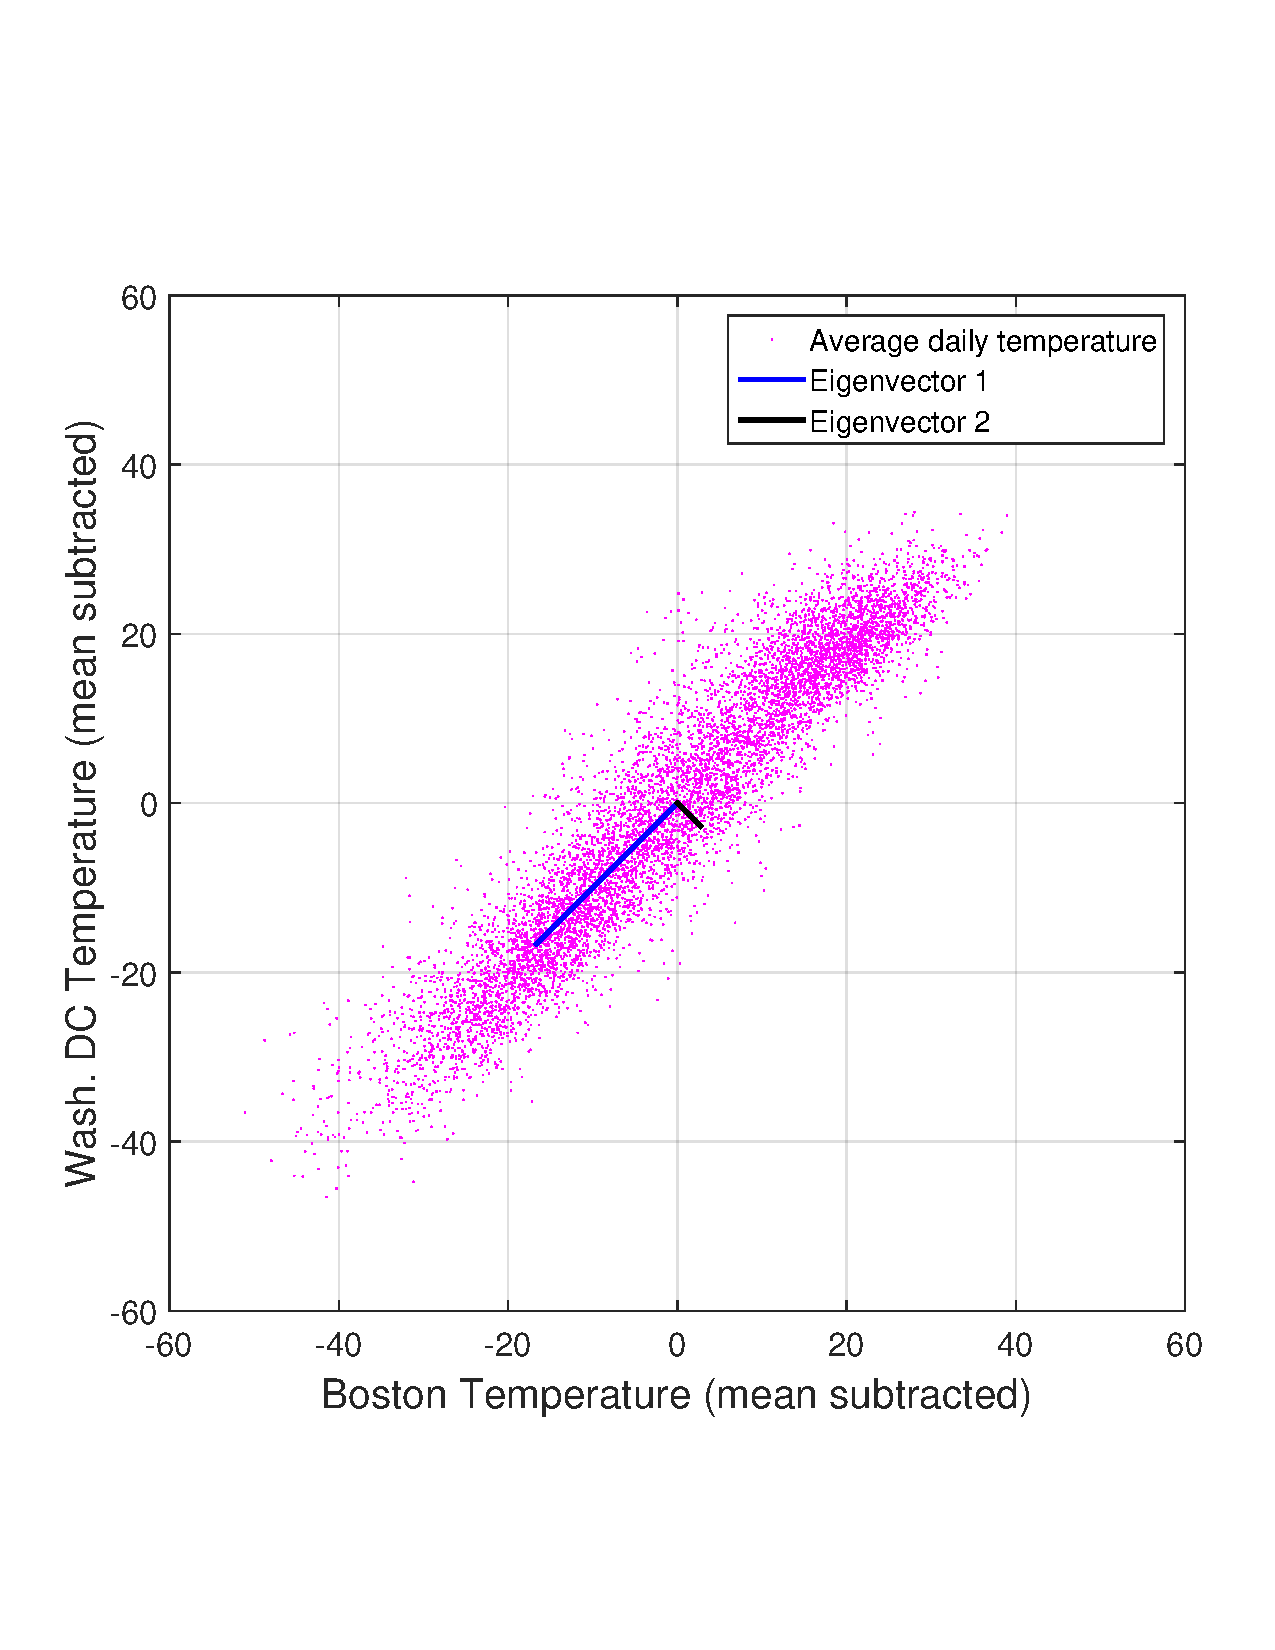
\includegraphics[width=0.75\textwidth]{FacesNight5/figs/BostonWashingtonCentered.pdf}
\captionof{figure}{Centered average daily temperatures of Boston vs Washington DC, with the eigenvectors of the covariance matrix. }
\label{figBostonWashington}
\end{center}


\begin{prob}\label{dataCovarianceQuestion} 
In this next problem, we are going to visualize how the eigenvectors of covariance matrices can tell us about the directions of most variation in 3D data. Load the file \texttt{temps\_bos\_sp\_dc.mat} in MATLAB. This file will load 21 years of temperature values for Boston, Sao Paolo and Washington DC. Treat the temperatures of Boston, Sao Paolo, and Washington DC for a given day as a point in a 3D space.
    \begin{enumerate}
    \item Subtract out the mean temperature of each city from the daily temperature data.
    \item Make a 3D scatter plot of the data points with the means subtracted out. You will find MATLAB's \texttt{plot3} function useful. You may wish to use the \texttt{'MarkerSize'} argument for \texttt{plot3} with a marker size of 0.1 or less to make the plots clearer.
    \item Construct a covariance matrix for the data and compute its eigenvectors.
    \item On the same axes, using \texttt{quiver3}, or \texttt{plot3}, plot the eigenvectors scaled by the square-root of their corresponding eigenvalues. Use \texttt{grid on} to draw grid lines on the axes to improve your visualization.
        \item Using the rotate 3D button on the figure window, rotate the image around to see how the eigenvectors tell you about the variation in the data.
    \end{enumerate}
\end{prob}
\begin{sol}
\begin{enumerate}
    \item \texttt{bn=b-mean(b);sn=s-mean(s);wn=w-mean(w);}
    \item \texttt{plot3(bn,sn,wn,'.','MarkerSize',0.1)}

\texttt{xlabel('Boston temperature (mean subtracted)')}

\texttt{ylabel('Sao Paolo temperature (mean subtracted)')}

\texttt{zlabel('Wash. D.C. temperature (mean subtracted)'}
\item \texttt{A=1/sqrt(length(b)-1)*[bn,sn,wn];}

\texttt{R=A'*A;}

\texttt{[V,D]=eig(R)}
\item \texttt{plot3(bn,sn,wn,'.','MarkerSize',0.1)}

\texttt{Vs=V.*sqrt(diag(D))}

\texttt{hold on}

\texttt{plot3([0,Vs(1,1)],[0 Vs(2,1)],[0 Vs(3,1)],'LineWidth',2)}

\texttt{plot3([0,Vs(1,2)],[0 Vs(2,2)],[0 Vs(3,2)],'LineWidth',2)}

\texttt{plot3([0,Vs(1,3)],[0 Vs(2,3)],[0 Vs(3,3)],'LineWidth',2)}

\texttt{grid on}

\texttt{axis equal}

See Figure \ref{temps}, which has the first eigenvector clearly aligned with the direction of greatest variation.

\begin{center}
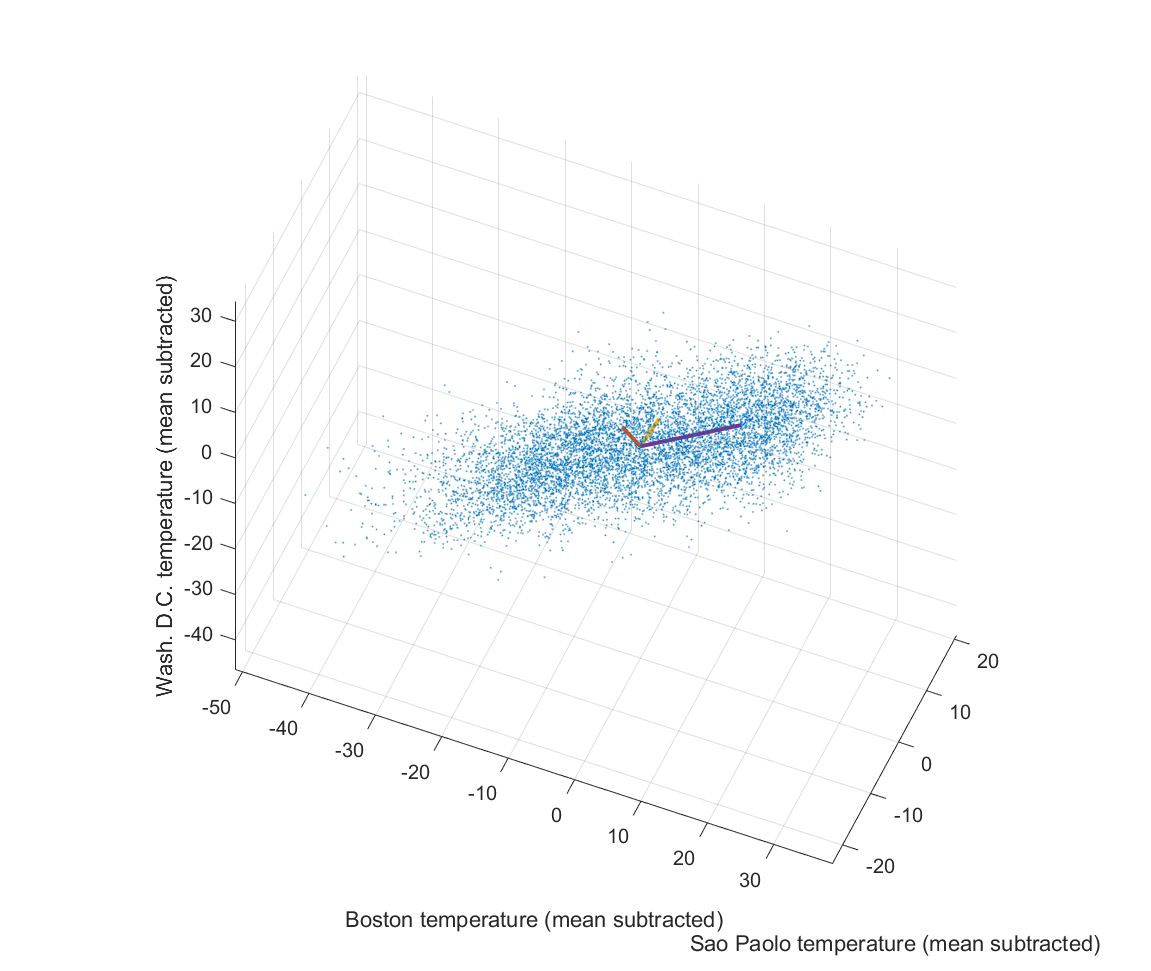
\includegraphics[width=0.75\textwidth]{FacesNight6/figs/tempplot.png}
\captionof{figure}{Temperatures and eigenvectors.}
\label{temps}
\end{center}
\end{enumerate}
\end{sol}

\section{Diagnostic Quiz}
Please see Canvas for the quiz questions.

\pagebreak
\shipoutAnswer
%LV end insert content from N7